%%%

\graphicspath{ {Figures/} }

\title{Numerical Programming 1 (CSE)\\Lecture Notes}
\author{Tommaso Bianucci\\\small{\texttt{bianucci <at> in.tum.de}}}
\date{\today}

\begin{document}
\maketitle
% \frontmatter
% \listoftodos
% \newgeometry{top=4cm}
\tableofcontents
% \restoregeometry
\section{Intro}
For this course, focus is on the math-details of computation and computational problems.

Algorithms will be sketched in MATLAB language, but it is also suggested to have a look at \href{http://www.julialang.org}{Julia}.

%EOF
 
% \mainmatter
\section{Basics}
\subsection{Floating point numbers}
Representing real numbers on a machine having finite resources is a non-trivial problem, in fact it is impossible to represent all of the infinite real numbers.

However, problems can arise even from a finite subset of them. Let's take for example \emph{irrational} numbers, such as $\pi$: irrational means they can't be represented as a fraction of two integers, which in turn means they have an infinite number of digits which don't repeat on any pattern. Storing all the digit of a single irrational number would then require \emph{infinite} space, which is impossible.

But also rationals are problematic: you can easily get an infinite number of digits (as with $\frac{2}{3} = 0.\overline{6}\,$) and on the other end you cannnot keep storing them as fractionals (i.e. couples of integers) since numerator and denominator can quickly become unmanageable in size.

The standard solution for this problem is to use the \emph{floating point} representation, wich allow us to express a subset of \RR on machines.
\begin{Def}
	Given a \emph{basis} $b \in \NN$, a range of possible \emph{exponents} $[e_{min}, e_{max}] \subset \NN$, a \emph{precision} $p \in \NN$ and a \emph{sign} $s \in \{0,1\}$, we can define a floating point number as a number $a_{fp} \in \RR$ which can be expressed in the form of:
	\begin{equation}
		a_{fp} = (-1)^s \cdot m \cdot b^e
	\end{equation}
	where
	\begin{equation*}
		e \in [e_{min}, e_{max}]
	\end{equation*}
	and there exist $m_0,m_1,\ldots,m_{i-1} \in [0,b-1]$ such that
	\begin{equation*}
		m = m_0 b^0 + m_1 b^{-1} + \ldots + m_{p-1} b^{-(p-1)}
	\end{equation*}
\end{Def}

With a notation abuse we can say that floating point numbers are in the form of:
\begin{equation*}
	(-1)^{s} \cdot m_0.m_1m_2 \ldots m_{p-1} \cdot b^e
\end{equation*}

\begin{Rem}
	In case we have $m_0 = 0$, \todo{Is it with a 0 or with a 1? I need to check} we say the representation is \emph{normalized}\footnote{Which is nothing else than the scientific notation of a number.}.
\end{Rem}

\begin{Rem}
	This notation obviously has limits on the maximum and minimum non-zero magnitude which can be represented. They can be obtained respectively by using the maximum possible mantissa and exponent or the minimum possible non-zero mantissa and exponent.

	Increasing a number above the upper limit leads to an \emph{overflow} and decreasing it below the lower limit leads to an \emph{underflow}.
\end{Rem}

\paragraph{The IEEE 754 standard}
Floating point numbers as they are commonly used in computers today are described in the IEEE 754 standard, which defines two types of floating point representations: the \emph{single precision}, using 32 bits (4 bytes), and the \emph{double precision}, using 64 bits (8 bytes).

Double precision is nowadays the \emph{golden standard} for computation, however single precision has gained more and more traction lately because they are commonly used in GPUs.

\begin{Def}[Double precision]
	Double precision floating point numbers are represented using 64 bits, allocated to sign, exponent and mantissa as follows\footnote{The base is 2.}:
	\begin{itemize}
		\item sign = 1 bit
		\item exponent = 11 bits
		\item mantissa = 52 bits
	\end{itemize}
\end{Def}

The IEEE 754 standard also defines some special values:
\begin{itemize}
	\item \emph{Inf}: $e = 2047$, $m = 0$.
	\item \emph{NaN}: $e = 2047$, $m \neq 0$.
\end{itemize}

\paragraph{Machine epsilon and rounding}
Machine epsilon, also called \emph{spacing}, is an important concept with floating point numbers, which is often used in thresholds.
\begin{Def}[Machine epsilon]
	Machine epsilon is defined as the smallest $\eps > 0$ such that, in floating point arithmetics, $1 + \eps \neq 1$.
\end{Def}
In other words, machine epsilon is the smallest possible mantissa.

When we have a number $a \in \RR$ and we want to represent it as a floating point number, we are often unable to represent it exactly. In this case, the best we can get is a number $\hat{a}$ ("$a$ hat") which we call the \emph{rounding} of $a$.

This $\hat{a}$ satisfies:
\begin{equation*}
	\frac{|a - \hat{a}|}{|a|} \leq \frac{\eps}{2}
\end{equation*}
Note that the quantity on the left-hand side of the inequality is called \emph{relative error} of $a$.

In conclusion, floating point arihmetic is very powerful because it allows for very fast and efficient computations, however the price that we pay for it is error.

\subsection[Problem conditioning]{Problem conditioning - The condition number}
\begin{Def}[Problem]
	A (mathematical) \emph{problem} is a map
	\begin{equation*}
		{f : X \rightarrow Y}
	\end{equation*}
	from an \emph{input} set $X$ to an \emph{output} set $Y$.
\end{Def}

If we now have a problem $f$ and we want to compute it in $x \in X$, to get $y = f(x) \in Y$ on a real machine, we need to necessarily approximate our values to floating point vaues: so we have $\hat{x}$ and we will compute $\hat{y} = f(\hat{x})$.

The question we now have is: how far will $\hat{y}$ be from $y$? This will surely depend on how good the approximation $\hat{x}$ of $x$ is, but also, and in a significant way, on how the problem itself intrinsically amplifies this error.
\begin{Ex}
	$f : x \mapsto 10^4 \cdot x,\quad Y = X = \RR$\\
	If $|x - \hat{x}| < \eps$, then
	\begin{dmath*}
		|y - \hat{y}| = |f(x) - f(\hat{x})| = 10^4 |x - \hat{x}| < 10^4 \cdot \eps
	\end{dmath*}
	So in this case we can see the error is \emph{amplified} by a factor of $10^4$, just by the problem itself and without accounting for computational errors.
\end{Ex}

This inherent error amplification can be quantified by defining:
\begin{Def}[Condition Number]
	The \emph{condition number} of a problem $f$ (at $x$) is the smallest $k_f(x) > 0$ such that
	\begin{equation*}
		\llb y - \hat{y} \rrb \leq k_f(x) \llb x - \hat{x} \rrb
	\end{equation*}
	where $y = f(x)$, $\hat{y} = f(\hat{x}$ and $\llb \cdot \rrb$ denotes a way to measure the error\footnote{Which is typically the relative error: $\llb x - \hat{x} \rrb = \frac{|x - \hat{x}|}{|x|}$}
\end{Def}
\begin{Ex}[$k_+$]
	The condition number of addition:
	\begin{equation*}
		{f : (x_1, x_2) \in \RR \mapsto x_1 + x_2 \in \RR}
	\end{equation*}
	\begin{dmath*}
		\llb y - \hat{y} \rrb = \frac{|y - \hat{y}|}{|y|}
		= \frac{|(x_1 + x_2) - (\hat{x_1} + \hat{x_2})|}{|x_1 + x_2|} \cdot \frac{|x_1| + |x_2|}{|x_1| + |x_2|} \\
		\stackrel{\triangle}{\leq} \frac{|x_1| + |x_2|}{|x_1 + x_2|} \cdot \frac{|x_1 + x_2| + |\hat{x_1} + \hat{x_2}|}{|x_1| + |x_2|}
		= k_+(x_1,x_2) \cdot \frac{||(x_1, x_2) - (\hat{x_1}, \hat{x_2})||_1}{||(x_1, x_2)||_1}
	\end{dmath*}
	We didn't prove that this is the minimum one, but it can be shown. So, considering $1$-norm relative error, we have:
	\begin{equation*}
		k_+(x_1,x_2) = \frac{|x_1| + |x_2|}{|x_1 + x_2|}
	\end{equation*}
\end{Ex}
\begin{Rem}
	This is usually not a problem, e.g. when $x_1$ and $x_2$ have the same sign. However we clearly see that, if we are subtracting two numbers with very similar magnitude, we may run into some troubles and get a $k_+(x_1,x_2) \gg 1$.
\end{Rem}
\begin{Rem}
	If the condition number of a given problem is $k_f$, in the output we lose $\approx log_{10}k_f$ decimal places of precision.
\end{Rem}

We can prove that other arithmetic operations, as $\times$ and $\div$ are well conditioned, with $k_\times = 2$ and $k_\div = 2$.

\begin{Lemma}
	In general if a problem $f : \RR^n \to \RR$ is differentiable, then it holds
	\begin{dmath*}
		k_f(x) = \frac{\scalprod{|\nabla f(x)|}{|x|}}{|f(x)|}
		= \frac{\sum_{i=1}^{n} |\partial_i f(x)||x_i|}{|f(x)|}
	\end{dmath*}
\end{Lemma}

\subsection{Stability of algorithms}
\begin{Def}[Algorithm]
	An algorithm is a finite sequence of arithmetic operations
	\begin{dmath*}
		f = f_n \circ f_{n-1} \circ \ldots \circ f_1 \circ f_0, \quad { f_i \in \{+,-,\times,\div\} }
	\end{dmath*}
\end{Def}
\begin{Def}[Implementation]
	Given an algorithm, its implementation is defined as
	\begin{dmath*}
		{ \hat{f}_n \circ \hat{f}_{n-1} \circ \ldots \circ \hat{f}_1 \circ \hat{f}_0, \quad \hat{f}_i \in \{\hat{+},\hat{-},\hat{\times},\hat{\div}\} }\\
		= \op{round} \circ f_n \circ \ldots \circ \op{round} \circ f_0
		= \hat{f}
	\end{dmath*}
\end{Def}
\begin{Rem}
	Given a problem, its decomposition into algorithms is not unique.
\end{Rem}
\begin{Rem}
	The choice of the algorithm has to be considered very carefully, since if some of its operations are badly conditioned we may obtain a significant error amplification even if the problem itself is well conditioned. This is the concept of \emph{stability} of an algorithm.
\end{Rem}
\begin{Def}[Stability]
	Given a problem $f$, an algorithm $\hat{f}$ for $f$ is said to be \emph{stable} if
	\begin{equation*}
		\llb f(x) - \hat{f}(x) \rrb \approx k_f(x) \cdot \eps
	\end{equation*}
	and \emph{unstable} if
	\begin{equation*}
		\llb f(x) - \hat{f}(x) \rrb \gg k_f(x) \cdot \eps
	\end{equation*}
\end{Def}
\begin{Rem}
	The intuitive meaning of stability is that if an algorithm is stable, its error amplification is in the same order of that of the theoretical conditioning of the problem. However if the algorithm is unstable, we have an error amplification wich is much greater than what it could be theoretically achievable.
\end{Rem}

\subsection[Notes on norms]{Notes on norms, matrix norms and induced matrix norms}
\begin{Def}[Norm]
	A (vector) norm is a function
	\begin{equation*}
		||\cdot|| : \RR^n \to \RR^+
	\end{equation*}
	satisfying all the following properties:
	\begin{enumerate}
		\item $||v|| = 0 \iff v = 0$
		\item $||\alpha v|| = |\alpha|\cdot||v||,\,\forall\, \alpha \in \RR$
		\item $||v + w|| \leq ||v|| + ||w|| \quad$ (triangle inequality, $\triangle$)
	\end{enumerate}
\end{Def}
\begin{Def}[Matrix norm]
	A matrix norm is symply a function
	\begin{equation*}
		||\cdot|| : \RR^{n \times m} \to \RR^+
	\end{equation*}
	which satisfies the three norm properties.
\end{Def}
\begin{Def}[Induced matrix norm]
	Given any vector norm $||\cdot||$ on $\RR^n$ and $\RR^m$, we can define, for matrices in $\RR^{n \times m}$, the corresponding induced norm as
	\begin{dmath*}
		||A|| \definedas \max_{v \neq 0} \frac{||Av||}{||v||} = \max_{||v|| = 1} ||Av||
	\end{dmath*}
\end{Def}
\begin{Ex}[Common induced norms]
Some examples of commonly used induced matrix normas are:
\begin{enumerate}[(a)]
	\item 	Vector $1$-norm induces the \emph{column-sum norm}:
	\begin{dmath*}
		||A||_1 = \ldots = \max_{k=1,\ldots,m} ||a^{(k)}||_1
	\end{dmath*}
	\item 	Vector $2$-norm induces the \emph{spectral norm}:
	\begin{dmath*}
		||A||_2 = \ldots = \sqrt{\max_{j=1,\ldots,m} \lambda_j (AA^t)}
	\end{dmath*}
	\item 	Vector $\infty$-norm induces the \emph{row-sum norm}:
	\begin{dmath*}
		||A||_\infty = \ldots = \max_{k=1,\ldots,n} ||a_{(k)}||_\infty
	\end{dmath*}
\end{enumerate}
\end{Ex}
\begin{Rem}[Properties of induced norms]
	Induced matrix norms show the following sub-moltiplicativity properties:
	\begin{enumerate}
		\item $||Av|| \leq ||A||\cdot||v||$
		\item $||AB|| \leq ||A||\cdot||B||$
	\end{enumerate}
\end{Rem}
%EOF

\section{Linear Systems}
A linear system is a problem defined as follows: given $A \in \RR^{n \times n},\,b \in \RR^n$ we want to find, if possible, $x \in \RR^n$ such that $Ax = b$.

\subsection{Solvability}
If we consider $a^{(i)}$ the $i$-th column of matrix $A$, we can express the linear system as:
\begin{dmath*}
	Ax = a^{(1)}x_1 + a^{(2)}x_2 + \ldots + a^{(n)}x_n \stackrel{!}{=} b
\end{dmath*}

So a solution exists iff $b$ can be represented as a linear combination of columns of $A$, i.e. $b \in \op{span}(a^{(1)},\ldots,a^{(n)})$.
We already know that if $A$ has \emph{full-rank}\footnote{Its rank is the same as its dimension.}, then
\begin{equation*}
	\op{null}(A) \definedas \{ x \in \RR^n | Ax = 0 \} = \{0\}
\end{equation*}
so, by Grassmann's formula, $\op{dim}(Im(A)) = n$, therefore $b \in \op{span}(a^{(1)},\ldots,a^{(n)})$.

From now on, we will typically assume $A$ to be full rank.

\paragraph{How to compute a solution}
\todo{This is actually nonsensicle here, we should move it to where we actually talk about solving.}We may be tempted to proceed the naive way: $Ax = b \implies x = A^{-1}b$, but this turns out to be a very bad idea because:
\begin{itemize}
	\item Inverting a matrix in practice requires solving $n$ linear systems of the form $Ax = e_i$.
	\item Matrix inversion can be unstable.
\end{itemize}

\subsection{Conditioning of linear systems}
Let's see a simple $2 \times 2$ linear system, to get an idea on why resolution of linear system can be well or badly conditioned to different degrees. Consider:
\begin{align*}
	\begin{cases}
		a_{11} x_1 + a_{12} x_2 &= b_1\\
		a_{21} x_1 + a_{22} x_2 &= b_2
	\end{cases}
\end{align*}
In the ideal world, the solution of each equation is a mono-dimensional sub-space, i.e. a line. If we look at the intersection of these two lines, which is the combined solution of the linear system, we get a single point (a null-dimensional space).

However, if we take into account representation error on both $b$ and $A$, we get that the solution to each equation is not just a line, but more like a strip. That is, all the possible lines which are near enough the theoretical solution to be rounded (in some sense) to it are possible solutions.
\begin{figure}[H]
	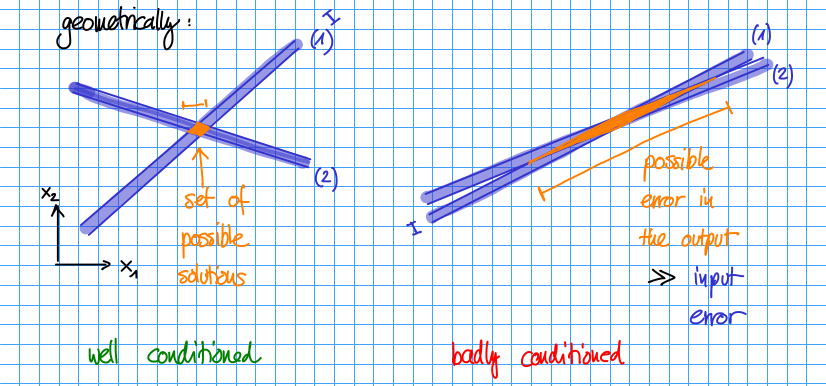
\includegraphics[width=\textwidth]{linSysConditioning}
\end{figure}
If we now consider the intersection of these two strips, we get an entire patch of the plane as possible solution set. We can see how the extent of this patch grows considerably the more the two solution strips tend to be parallel. This is, in simple terms, the conditioning of a linear system.
% EOF


% \backmatter
% \input{Chapters/08_Acknowledgements}
%%%% \nocite{*}
% \bibliographystyle{plain}
% \addcontentsline{toc}{chapter}{Bibliography}
% \bibliography{bibliography}

\end{document}
